\appendix{Specyfikacja interfejsów Lupus}\label{appendix:4}

Specyfikacja w formie elektronicznej znajduje się pod linkiem: \url{https://github.com/0x41gawor/lupus/blob/master/docs/spec/lupin-lupout.md}.

\subsection{Architektura}

\begin{figure}[!h]
    \centering 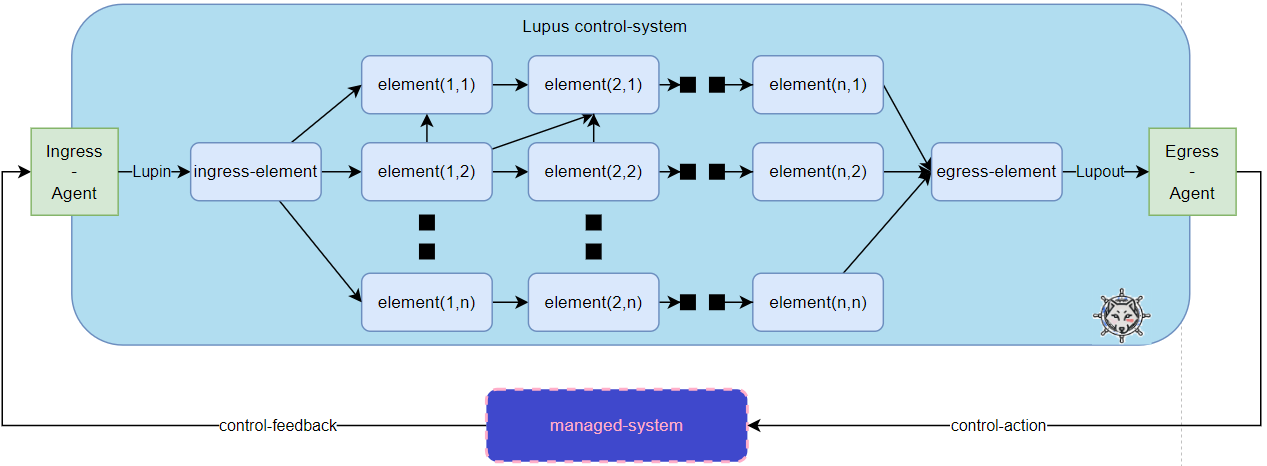
\includegraphics[width=1\linewidth]{a4-arch.png}
    \caption{Architektura Lupus}\label{fig:a4-arch}
\end{figure}

\subsection{Interfejs Lupin}

Projektant może zdefiniować wiele \textbf{Elementów Lupus}, połączonych na różne, skomplikowane sposoby. Musi jednak zdecydować, który z nich zostanie wywołany przez \textbf{IAgenta Ingress}. Taki element można nazwać \textbf{Element Ingress}. Lupus zaleca posiadanie tylko jednego Elementu Ingress.
Jeśli \textbf{Agent Ingress} chce zasygnalizować, że można zaobserwować nowy stan systemu zarządzanego (co oznacza, że musi zostać uruchomiona nowa iteracja pęli sterowania), musi zmodyfikować pole \texttt{Status.Input} w \textit{obiekcie API} \textbf{Elementu Ingress}. Wartość umieszczona w tym polu będzie reprezentować nowy \textbf{Aktualny Stan}.

Pole \texttt{Status.Input} w \textbf{Ingress Element CR} jest typu \texttt{RawExtension}, co oznacza, że podlega pod specyfikacje danych \\TODO załącznik daty

JSON przesłany w tym miejscu będzie stanowił \textbf{Dane} dla tego elementu.

Oprogramowanie implementuje interfejs \texttt{Lupin}, jeśli w pewnym miejscu swojego kodu wysyła żądanie HTTP do \textbf{kube-api-server}, które aktualizuje status \textbf{Elementu Ingress}, a dokładniej pole \texttt{input}. Wartość musi być obiektem JSON, który reprezentuje \textbf{Aktualny Stan} \textbf{Zarządzanego Systemu}. 

\subsection{Interfejs Lupout}

Punktem wyjścia z \textbf{Systemu Sterowania Lupus} jest ostatni \textbf{Element Lupus} czyli (\textbf{Element Egress}). Wysyła on swoje \textbf{finalne dane} (lub ich część) do \textbf{Agenta Egress}. \textbf{Egress Agent} musi przekształcić to wejście w \textbf{Akcje Sterowania}, wykonywaną bezpośrednio na \textbf{systemie zarządzanym}.

Oprogramowanie implementuje interfejs \texttt{Lupout}, jeśli implementuje serwer HTTP, który akceptuje wejściowe dane JSON i tłumaczy je na \textbf{Akcje Sterowania} wykonywaną na \textbf{Systemie Zarządzanym}. 

